\section{Experiments} \label{sec:experiments}

In the previous sections we have been going the through the theoretical
background of the different approaches we were going to make use of to classify
the provided MaCom data. However from this point the practical aspect will be in
focus. The following sections address what went into implementing the different
methods, and why their final structure and parameters are what they are. Not
only that, but each method will be tested against the external validation set
(C). This will leave us with a final set of candidate methods which is to be run
on the test dataset. Two of these will be the baseline method, and the other
two will be the best performing recurrent network, and the best performing
convolutional network.


\subsection{Baseline Methods} \label{subsec:baseline}

In this section we will go through the experiments performed in order to get
our baseline results. While many different features can be used when performing
\gls{NLP}, we chose the same features, as was used in \cite{US}, since they
span several several of the different linguistic layers. The linguistic layers
are different areas which all serve to describe a certain text. An example this
could be the character level layer, which as the name implies, focuses on the
individual characters used in a specific text. Other examples of this, could
be the sentence layer, that focuses on the sentences of the text, and the meta
layer, that focuses on things such as publishing/delivery date, and file format.
The features available to pick from in this case are:

\begin{itemize}
    \item Word-N-grams,
    \item Character-N-grams,
    \item Word Frequencies (word-1-grams),
    \item \gls{POS}-tag-N-grams, and
    \item Special-Character-N-grams,
\end{itemize}

Where an N-gram describes the combinations of sequential elements of size n. In
the case where that element is characters, and n is 3, the string "hello" would
produce the character-3-grams "hel", "ell" and "llo". This also means that a
feature such as word frequencies can be considered word-1-grams.

\gls{POS} tags, refer to the grammatical class a certain words belongs to, such
as nouns and adjectives. In order to extract these we made use of a POS-tag
extractor, provided by \cite{polyglot}.

For all of these experiments a Danish third party corpus, provided by
\texttt{NLTK}\footnote{\url{http://www.nltk.org/index.html}}, was used as the
basis for all the feature extraction, as was done in \cite{US} as well. This
corpus consists of 22,476 sentences, and 563,358 words.

The actual implementation of both the \gls{SVM} and the Extended Delta method,
very closely resembles the implementation used in \cite{US}. There is however a
very big difference, with the actual application of the delta method. Contrary
to the scenario in \cite{US}, where PAN data was used, there is not an instance
where we only have 1 text per author. As such the original version of the
delta method can be used.\cite{evert2015towards} This is where, when given a
new text $x$ supposedly written by an author $\alpha \in \mathcal{A}$, his
texts $T_\alpha$ are extracted, and so is a set of texts no written by him
$\overline{T}_\alpha$ where $|\overline{T}_\alpha| = |T_\alpha|$. The text,
along with a negative sample text $z$, we know now to be written by $\alpha$ is
given to a \gls{KNN} classifier, which determine if $x \in T_\alpha$ and $z \in
\overline{T}_\alpha$.

\subsubsection{Feature Selection *Under Reconstruction*}

The larger part of the experiments performed using the baseline methods, was
centered around parameter tuning. Not only parameter as the K in the extended
delta method, but also the feature supplied to the method. Other methods such
as random forest has a built in filter for bad and noisy feature. This is not
the case for both the \gls{SVM} and extended delta method, who does performs any
kind of quality analysis of the feature they are given, making them susceptible
to the negative influences these features include. It is for this reason that
we chose to select the features for them, rather than just having them use the
entire set available to them.

Contrary to our previous work made in \cite{US}, this process did not
consist of trying out some random selection of features, but rather
a more systematic approach was used.

However, before starting to do that, a feature set had to be created
first. In order for us to find the very best set of features, we wanted
to create a very large initial feature set, so as to increase our search space.
The corpus used had the following quantities of the different features.

\begin{itemize}
    \item Word-2-grams - 188,472
    \item Character-2-grams - 2,178
    \item Word Frequencies - 27,535
    \item \gls{POS}-tag-2-grams - 219
    \item Special-character-2-grams - 524
\end{itemize}

The quantities here are of course very large due to the size of the corpus,
and will continue to rise as N increases. Rather than extracting all
of those feature from our texts, we chose to focus on the N-grams
with highest frequency, as we would reach a point where a specific N-gram
determined to be in the corpus, would be unique that same corpus, making it
irrelevant for new texts, not associated with the corpus.

Using the quantities listed above as inspiration, a feature set of 4950
features was produced, containing

\begin{itemize}
    \item The 500 most frequent words,
    \item The 500 most frequent word-N-grams for $N \in \{2,3,4\}$,
    \item The 300 most frequent character-N-grams for $N \in \{2,...,10\}$,
    \item The 50 most frequent \gls{POS}-tag-N-grams for $N \in \{3,4\}$, and
    \item The 50 most frequent special-character-N-grams for $N \in \{2,3,4\}$.
\end{itemize}

The selection the quantities, was based on the number available in the corpus,
listed earlier. The number of different character N-grams we extracted was based
on the amount used in \cite{aalykke2016}. They found out that char-8-grams
worked very well on MaComs data, which is the reason why we chose to include
char-N-grams with a N spanning the values from 1 to 10. Looking at the results
from \cite{US}, revealed that the N in word-N-grams reach a value of 4,
the probability of that sequence actually occurring drastically reduced,
and with it its' overall impact. A similar thing could be seen with the
special-character-N-grams, where an increase in N, would not contribute
anything. The reason for the small amount of \gls{POS}-tag-N-grams was that
they were a really big burden computationally, as such a reduction in possible
N-values had to be made.

It should be noted that the work done in \cite{US} was done on English
texts rather than Danish as is the case in this paper. While there there is
a discernible between the languages the overall difference is not actually
that far. This is a point also made in \cite{konstantin:2000}, where
using a lexical distance equation he computed the distance between all
the European languages. A upgraded figure of his finding can be found
here\footnote{\url{https://bit.ly/1BOMe9l}}. This model reveal
that Danish end English are in fact not so lexical different, which makes sense
as the both derive from the germanic branch of the indo-European language
family.

These features were extracted from the data-set (I) described in Section
\cite{sec:data}. The distribution of the texts over authors in this data-set is
not very evenly spread. As such, the random selection of random opposing authors
has a certain amount of bias towards the authors with a large amount of texts
compared to the test.

Having the features, we could start doing our feature selection. This whole
process proved very expensive computationally. Having to check every combination
of 5000 features, simply was not feasible. It was for that reason we opted for a
greedy algorithm in combination with the drastically small data-set (I) instead.

The greedy algorithm works as described by \cite{kanDeng}, which is a simple
forward feature selection. Having out previously created feature set, we loop
through each single feature, validating its' accuracy when applied to each
$\alpha \in \mathcal{A}$, where in this case $\mathcal{A}$ is the dataset
(I). As eluded to earlier, this consists of fetching $T_{\alpha}$ and a set
$\hat{T}^{(I)}_{\alpha}$, where $|\overline{T}_\alpha| = |T_\alpha|$. Using
this set of positive and negative cases, we make use k-fold cross validation
to determine the performance of the feature for that author. This is done for
all authors, and when averaged we have the performance of that single feature.
This process is then repeated for all features. The best performing feature is
then added to out candidate set of features. The next iteration we loop through
all the feature again, but we validate against each feature in combination with
the already selected features. This process is repeated until a set number of
features are selected. At this point we determine at which point we had the best
candidate set, and use that hence fourth.

Even this greedy approach proved to be very time consuming. As such, we only did
as described and found the best features, but left out the hyper-parameters C,
and $\gamma$ for the SVM, and K and the distance metric for the extended delta
method. These hyper-parameters were selected through a separate process
which will be described in a later section.

Due to the increased run-time when using leave one out cross validation, we had
to make use of some other model selection approach. Under normal circumstances,
normal X-fold cross validation would work out fine, but a complication arose
when doing this with the extended delta method, which yielded normal cross
validation unfit for that specific classifier. The reason for this was that
there was a scenario where an unlucky split of folds would cause a lot of error.
A generic example of this would be if we had the 2 class training set consisting
of 6 value, evenly split between the 2 classes. In the case where we split those
6 values into 3 folds, there is a chance that a fold contains two value of the
same class, which means that if $K = 3$ in our case, both of those wont ever be
able to classified correctly as there is only 1 of that class in the training
set. As such, stratified K fold cross validation is used instead, as it uphold
the class distribution in its' folds. While this problem would not plague the
SVM classifier, we also opted the stratified K fold cross, so we would more
directly compare the feature selection of the two models.

For both the \gls{SVM} and Extended Delta method, we ran this algorithm
until 450 features were selected. The SVM performed its' feature
selection using the default RBF kernel, a C with value 1, and $\gamma =
\frac{1}{\text{n\_features}}$. Due to some authors having below 3 texts,
the default K value of \gls{KNN}s K parameter was set to 3 for the feature
selection.

The results of both the SVM and the Extended Delta method feature selection can
be seen in Figure \ref{fig:fs_results}. We got that the best number of selected
feature were 220 for the SVM and 4 for the Extended Delta Method, scoring an
accuracy of [TODO:Res] and [TODO:Res] respectively.

\begin{figure}
    \centering
    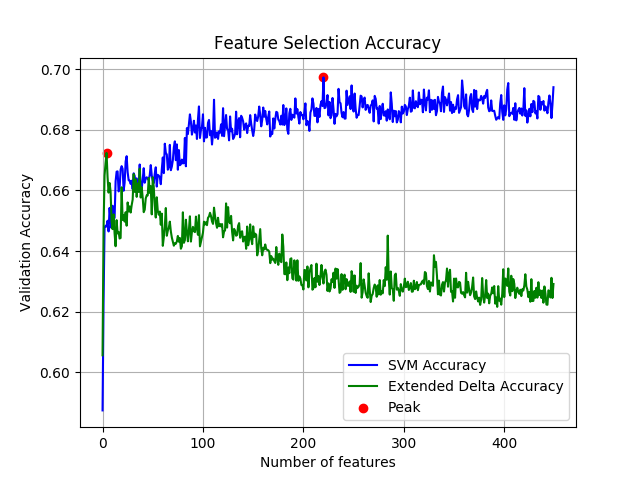
\includegraphics[scale=0.8]{./pictures/experiments/feature_selection.png}
    \caption{The process of the greedy feature selection of the SVM and the Extended Delta Method}
    \label{fig:fs_results}
\end{figure}


\subsubsection{Hyper Parameter Selection}

As mentioned in the previous section, due to computational time, we were unable
to do the hyper parameter selection parallel with the feature selection.
For that reason we chose to split it up, selecting our features first, and the
fine tuning our parameters based on those selected features.

This means that our implementation very closely mimics the one used in the
previous example. On both cases we start out with two lists of possible hyper
parameter values:

\begin{align}
    \text{SVM} &:
    \begin{array}{lr}
        C=\{10^{-3}, 10^{-1}, 10^{1}, 10^{3}, 10^{5}, 10^7\}\\
        \gamma=\{10^{-3}, 10^{-1}, 10^{1}, 10^{3}, 10^{5}, 10^7\}
    \end{array} \\
    \text{Extended Delta} &:
    \begin{array}{lr}
        p=\{1,2,3,4,5\}\\
        K=\{1,3,5,7,9,11,13,15\}
    \end{array}
\end{align}

The one parameter yet to be explained i $p$, which refers to the p in the
minkowski distance,

\begin{equation}
    D(X,Y) = \left(\sum_{i = 1}^n |x_i - y_i|^p\right)^{1/p},
\end{equation}

where $p=1$ and $p=2$ is the manhattan and eucledian distance respectively.

The following was perform on the data-set (J) as this, contrary to the feature
selection is more computationally efficient.

We perform a grid search over all these parameters. For each variation of the
hyper parameters we average the performance of the method over all unique
authors in the training set, in a manner very similar to the feature selection.
We make use of the same 3-fold stratified cross validation, and arrange each
authors with set of opposing set of text, amounting to the same number he has
written himself. The accuracy of each parameter configuration can be seen
in Table \ref{sec:ed_feat} for \gls{KNN}, and Table \ref{sec:svm_feat} for
\gls{SVM}.

\begin{table}[h]
    \centering
    \caption{The results from performing a grid search of the p and K parameter
        of the \gls{KNN} algorithm}
    \label{table:KNN}
    \begin{tabular}{|c|ccccc|}
        \hline
        \backslashbox{$K$}{$p$} & 1 & 2 & 3 & 4 & 5 \\\hline
        1 & \textbf{0.630} & 0.603 & 0.588 & 0.577 & 0.570\\
        3 & 0.628 & 0.589 & 0.572 & 0.565 & 0.555        \\
        5 & 0.621 & 0.576 & 0.559 & 0.549 & 0.545        \\
        7 & 0.612 & 0.564 & 0.546 & 0.537 & 0.533        \\
        9 & 0.600 & 0.554 & 0.537 & 0.527 & 0.524        \\
        11 & 0.587 & 0.542 & 0.527 & 0.520 & 0.517       \\
        13 & 0.581 & 0.537 & 0.524 & 0.517 & 0.514       \\
        15 & 0.571 & 0.532 & 0.519 & 0.514 & 0.512      \\\hline
    \end{tabular}
\end{table}

\begin{table}[h]
    \centering
    \caption{The results from performing a grid search for C and gamma, of the
        \gls{SVM} algorithm}
    \label{table:SVM}
    \begin{tabular}{|c|cccccc|}
        \hline
        \backslashbox{$C$}{gamma} & $10^{-3}$ & $10^{-1}$ & $10^{1}$ & $10^{3}$ & $10^{5}$ & $10^{7}$ \\\hline
         $10^{-3}$ & 0.626 & 0.626 & 0.626 & 0.641 & 0.558 & 0.500\\ 
         $10^{-1}$ & 0.626 & 0.626 & 0.626 & 0.641 & 0.558 & 0.500\\ 
         $10^{1}$  & 0.626 & 0.626 & 0.626 & \textbf{0.689} & 0.576 & 0.501\\ 
         $10^{3}$  & 0.626 & 0.626 & 0.681 & 0.687 & 0.576 & 0.501\\ 
         $10^{5}$  & 0.626 & 0.680 & 0.678 & 0.687 & 0.576 & 0.501\\ 
         $10^{7}$  & 0.674 & 0.678 & 0.678 & 0.687 & 0.576 & 0.501 \\\hline
    \end{tabular}
\end{table}

It is at this point we grab the data-set (C), our external
validation set. While applying these finely tuned methods to a validation set
wont change anything in terms of the parameters we have selected, it will give
us the ability to gauge the accuracy of our methods when applied to a new, never
before seen, test-set.

\begin{center}
\begin{verbatim}
Extended Delta Validation Accuracy: [TODO:RES]
SVM Validation Accuracy:  [TODO:RES]
\end{verbatim}
\end{center}


\subsection{Deep Learning}

In the prediction system from Definition \ref{def:prediction_system} we needed
a function $f$ that takes two texts and returns the probability that those
texts are written by the same author. As described earlier Siamese Neural
Networks are well suited for comparing objects. In this Section we describe
the experiments we performed with different networks architectures and we
will present three different networks. The three networks are \gls{conv-char-NN}
in Section \ref{subsubsec:conv_char_nn}, \gls{conv-char-word-NN} in Section
\ref{subsubsec:conv_char_word_nn}, and \gls{rec-sent-NN} in Section
\ref{subsubsec:rec_sent_nn}.

The data we trained our networks on is described in Section \ref{sec:data}. We
trained the networks on the (G) dataset that contains 3000 authors. We used
early stopping based on a validation dataset (H) that contains 500 authors.
Through experimentation we found that the validation dataset had to contain
completely different authors than the training dataset. In the beginning of
our project we had a validation set that contained different problem instances
(two texts to compare) from the training set but contained some of the same
authors. That lead to the validation set not being a very good estimate of the
networks performance on different authors than the ones seen during training.
The networks were therefore overfitting on the specific authors and we could not
see that in the validation datasets accuracy. All accuracy graphs shown in this
Section are based on a validation dataset with 500 completely unseen authors.

The general structure of our networks will be that they take two texts as input.
The texts are first embedded into a format that can be used by the network.
Then the texts are transformed into two sets of features representing the text
via a weight sharing network. Then the text representation will be combined
in some way and a dense network will take the combined representations and
decide whether or not the texts are written by the same author. We call the
different parts of the network \textit{Embedding}, \textit{Feature Extraction},
\textit{Combining} and \textit{Decision}.

When we show graphs of the networks we have produced we use specific names for
different layers in the networks. A glossary of the layer names and paramters of
the layers are shown in Table \ref{tab:glossary}.

\begin{landscape}
    \begin{table}
        \centering
        \caption{Glossary used when performing experiments, and creating their
            associated models.\cite{chollet2015keras}}
        \label{tab:glossary}
        \begin{tabular}{|L{3cm}|L{9cm}|L{11cm}|}
            \hline
            \multicolumn{1}{|c|}{\textbf{Layer}}                               &
            \multicolumn{1}{|c|}{\textbf{Description}}                         &
            \multicolumn{1}{|c|}{\textbf{Actively Used Parameters}}           \\
            \hline

            Input                                                              &
            Serves as the entrypoint of the network, by receiving a set of
            texts and feeding it trough the network.                           &
            \begin{minipage}[t]{\linewidth}
            \begin{compactdesc}
                \item[Shape] The dimensions of each sample give to the input.
            \end{compactdesc}
            \end{minipage}                                                    \\
            \hline

            Embedding                                                          &
            Taking in an encoded sample, it produces a dense vector
            representation for each different. More details can be found in
            Section \ref{subsubsec:layers}.                                    &
            \begin{minipage}[t]{\linewidth}
            \begin{compactdesc}
                \item[Input Dim] Size of vocabulary.
                \item[Output Dim] Size of vector used to represent embedding.
            \end{compactdesc}
            \end{minipage}                                                    \\
            \hline

            Convolutional                                                      &
            Applies convolution to the data it recieves according to the
            decription, found in Section \ref{subsubsec:layers}.               &
            \begin{minipage}[t]{\linewidth}
            \begin{compactdesc}
                \item[Filters] Dimensionality of the output, ie. number of
                    filter from the convolution.
                \item[Kernel Size] Integer or list describing size of
                    convolution window.
                \item[Strides] Stride length of the convolutional window.
                \item[Activation] The activation function to be applied after
                    the convolution.
            \end{compactdesc}
            \end{minipage}                                                    \\
            \hline

            Global Max Pooling                                                 &
            Extracts the maximum value from each of the provided data          &
            No parameters.                                                    \\
            \hline

            Concatenation                                                      &
            As the name suggests, this layers simply concatenates the data it
            receives from different layers                                     &
            No parameters.                                                    \\
            \hline

            Merge                                                              &
            Merges its inputs, using a specified function to generate a single
            output.                                                            &
            \begin{minipage}[t]{\linewidth}
            \begin{compactdesc}
                \item[Function] The function used to merge the recieved data.
            \end{compactdesc}
            \end{minipage}                                                    \\
            \hline

            Dense                                                              &
            A simple fully connected layer, taking in data and applying the
            function described in Section \ref{sec:neurons}.                   &
            \begin{minipage}[t]{\linewidth}
            \begin{compactdesc}
                \item[Units] Number of neurons in in the layer.
                \item[Activation] The activation function to be applied.
            \end{compactdesc}
            \end{minipage}                                                    \\
            \hline

            Dropout                                                            &
            Drops a fraction it receives, with the goal of preventing
            overfitting.                                                       &
            \begin{minipage}[t]{\linewidth}
            \begin{compactdesc}
                \item[Rate] The fraction of data it receives dropped.
            \end{compactdesc}
            \end{minipage}                                                    \\
            \hline

            Lambda                                                             &
            Applies a specified function to the input it receives              &
            \begin{minipage}[t]{\linewidth}
            \begin{compactdesc}
                \item[Function] The function applied.
            \end{compactdesc}
            \end{minipage}                                                    \\
            \hline

            Reshape                                                            &
            Reshapes the data it receives.                                     &
            \begin{minipage}[t]{\linewidth}
            \begin{compactdesc}
                \item[Dim] Dimensionality to reshape to.
            \end{compactdesc}
            \end{minipage}                                                    \\
            \hline

            LSTM                                                               &
            A Long Short-Term Memory layer, which works according to the
            description in Section \ref{subsubsec:layers} is applied to the
            given data.                                                        &
            \begin{minipage}[t]{\linewidth}
            \begin{compactdesc}
                \item[Unit] Number of neurons in the layer.
            \end{compactdesc}
            \end{minipage}                                                    \\
            \hline
        \end{tabular}
    \end{table}
\end{landscape}


\subsubsection{\glsdesc{conv-char-NN}}
\label{subsubsec:conv_char_nn}

The idea behind network \gls{conv-char-NN} is that we wanted to use convolutions
to look for n-grams in texts. Traditional authorship verification/attribution
is based on carefully engineered n-grams that are compared between two texts
\cite{stamatos2009}. Instead of choosing the n-grams ourselves we wanted the
network to learn which features are important for the authorship verification
task. The features are learned through convolutions. The convolutions look
at some number of characters at a time and gives a single output for those
characters. Assume for example that the network has learned that the character
sequence "ould " is important for deciding the author of a text. Then we
expect the network to react strongly to character sequences that looks
like "ould ". We have illustrated such a convolutional filter in Figure
\ref{fig:convolution_text_example}.

\begin{figure}
    \centering
    \textbf{Convolutions for Text Feature Extraction}\par\medskip
    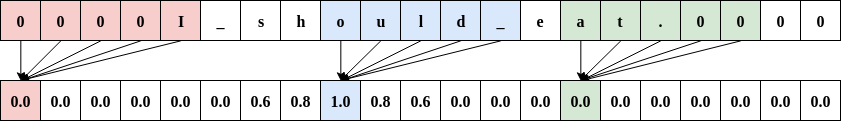
\includegraphics[width=\textwidth]{./pictures/experiments/convolution_example.png}
    \caption{Illustration of character level convolutions using a filter that
        looks for the character sequence "ould ". Notice that high values are
        produced when the characters the filter looks at match the characters it
        is looking for and low values are produced otherwise. We have
        illustrated 3 different filter locations but the filter is similarly
        placed in all possible locations. We have padded the text with zeros to
        get the same size output as input.}
    \label{fig:convolution_text_example}
\end{figure}

\begin{description}

    \item[Embedding:]

        The embedding takes as input a sequence of integers. Each different
        integer is a compact one-hot encoding of each character. The one-hot
        encoded character stream is embedded in a five dimensional space. The
        hope is that the layer will learn that similar characters should be
        placed close to each other in the output space and dissimilar characters
        should be placed far apart. The same embedding is performed on both of
        the input texts and the layer is therefore part of the Siamese part of
        the network.

    \item[Feature Extraction:]

        Features are extracted from the two texts via a layer of convolutions
        with different sizes. We use both convolutions with a window size of
        8 and convolutions with a window size of 4. We use 700 of size 8 and
        500 of size 4. We used a window size of 8 since \cite{aalykke2016}
        found that n-grams of size 8 worked the best for Danish texts and we
        also added 4 so the network could look at smaller n-grams as well.
        We used a stride of 1 such that each convolutional filter could
        observe all parts of the texts and give an output for each one. The
        convolutional part of the network also shares weights such that the
        same features are extracted from both the input texts. We use the
        \gls{ReLu} activation function for the reasons described in Section
        \ref{subsubsec:activation_functions}.

        After the convolutional layer we added a global max pooling layer. The
        layer takes the maximum output of each convolutional filter. We do that
        as the output size of the convolutional layer depends on the length of
        the input text. The output of the max pooling layer is $700 + 500 =
        1200$ numbers, one for each convolutional filter. That means that the
        network learns to extract 1200 different features from each text.

    \item[Combining:]

        The features of the texts are combined using the absolute difference
        function. As described each text is represented as a vector of 1200
        features and to combine them we subtract them from each other and take
        the elemtwise absolute difference.

    \item[Decision:]

        The decision part of the network consists of 4 dense layers each with
        500 neurons, a dropout layer and an output layer. The 4 dense layers
        also use the \gls{ReLu} activation function. The dropout layer is added
        just before the output layer and performs 30\% dropout to try to combat
        overfitting. The actual prediction is performed in the output layer.
        The output layer use the softmax function to return a probability
        distribution over the two possibilities that the texts are written by
        the same author and that they are written by different authors.

\end{description}

We have shown an illustration of the network in Figure \ref{fig:conv-char-NN}.
In the Figure we have illustrated the Siamese part of the network as a blue box.
The 4 phases of the network is not illustrated in the Figure but it should be
possible to find them by reading the description above. We trained the network
on the dataset described in the Section \ref{sec:data} and in the beginning
of this Section. We used the \gls{Adam} optimizer during the training of the
network. We used a learning rate of $\eta = 0.0005$, half of what was suggested
by \cite{DBLP:journals/corr/KingmaB14}. We did that as we had problems with
neurons dying during the training of the network otherwise. Other than the
learning rate we used the parameters suggested in the article. That is, the
remembering rates were set to $\gamma_1 = 0.9$ and $\gamma_2 = 0.999$. As the
error function we used the Categorical Crossentropy function described in
Section TODO. When we trained the network we were able to obtain a validation
accuracy of 0.71773 in epoch 6. The training accuracy continued rising but we
used early stopping since the validation accuracy had stopped improving. We
have shown a graph of the training and validation accuracies during training in
Figure \ref{fig:conv-char-NN-accuracies}. During the training we used minibatch
learning with a minibatch size of 8. We used a size of 8 as that was the largest
batch size that could fit in the GPUs memory. During the training we padded
all texts with zeros such that all texts in each batch had the same length. We
did that as it is required by Keras. We have shown the training and validation
accuracies during training in Figure \ref{fig:conv-char-NN-accuracies}.

\begin{figure}
    \centering
    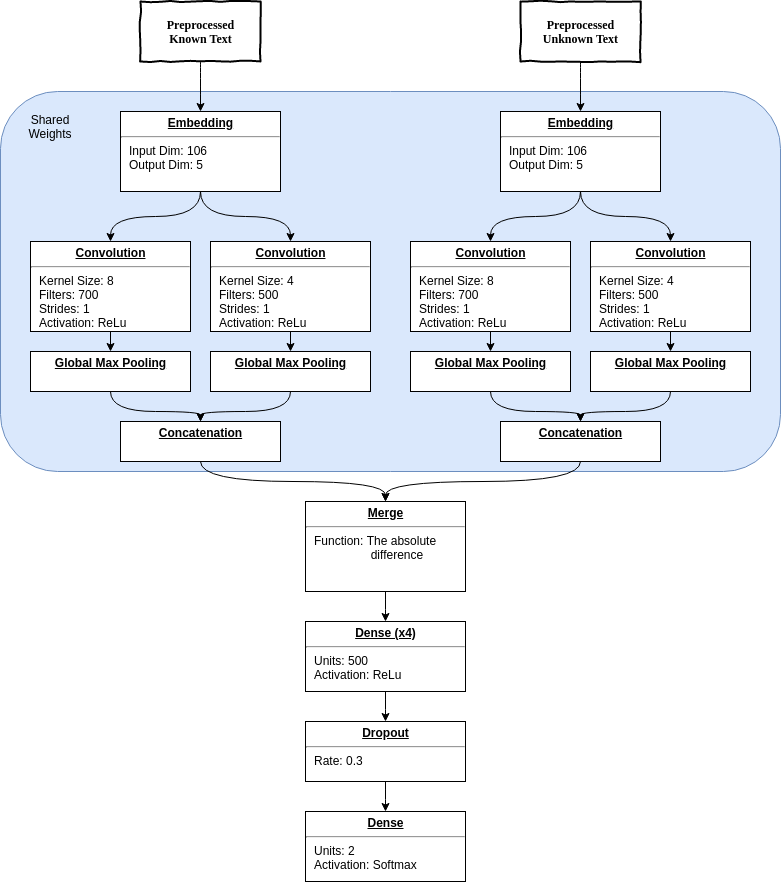
\includegraphics[width=\textwidth]{./pictures/experiments/conv_char_nn/model.png}
    \caption{The structure of network \gls{conv-char-NN}. Weights are
        shared by the embedding layers and the convolutional layers as shown by
        the blue box. The input to the network is at the top and the output is
        at the bottom. Information flows downwards through the layers. The final
        softmax layer produces a probability distribution over the two
        possibilities that the texts are either written by the same author or
        not.}
    \label{fig:conv-char-NN}
\end{figure}

\begin{figure}
    \centering
    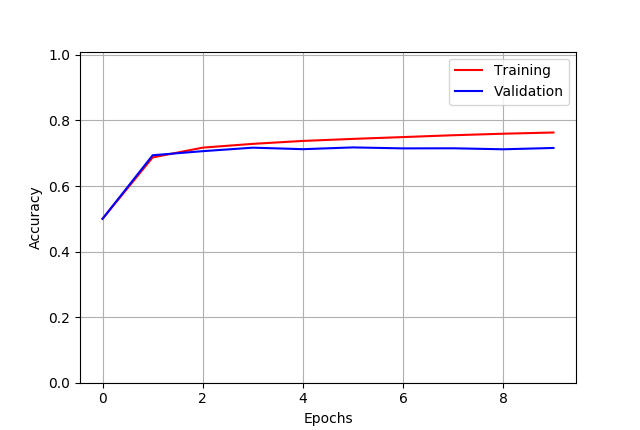
\includegraphics[width=\textwidth]{./pictures/experiments/conv_char_nn/training_accuracy.png}
    \caption{The training and validation accuracy of \gls{conv-char-NN} during
        training. Each epoch contains several thousand minibatches which is why
        the training and validation accuracies rises so much in the first
        epoch.}
    \label{fig:conv-char-NN-accuracies}
\end{figure}

To arrive at the network architecture described above we experimented with
several similar architectures. We started with a network that used,

\begin{description}

    \item[Embedding:]

        Same as described above.

    \item[Feature Extraction:]

        1000 convolutional filters of size 10.

    \item[Combining:]

        Instead of the absolute difference we used a concatenation of the
        feature vectors extracted from the two texts. If we let the extracted
        features of the first text be $T_{1,i}$ and the extracted features of
        the second text be $T_{2,i}$ then $T_{1,0}$ and $T_{2,0}$ correspond
        to the same feature extracted from the two texts. The concatenation
        combining function would then compute,

        \begin{equation}
            combine(T_1, T_2) \rightarrow \left(
                T_{1,0}, T_{1,1}, \dots, T_{1,n}, T_{2,0}, T_{2,1}, \dots, T_{2,n}
            \right)^T.
        \end{equation}

    \item[Decision:]

        We used a small dense network with only a single hidden layer of 500
        neurons. The output layer was similar to the one described above.

\end{description}

The network gave promising results which is why we continued working with it but
it quickly overfitted on the training data so we added some dropout. Like in
the network presented above we added the dropout layer just before the output
layer and used 30\% dropout. That regularization allowed the training accuracy
and validation accuracy to follow each other for more epochs making the final
validation accuracy better.

We changed the combining function from a concatenation to a absolute difference
since the network would then not have to learn which features belonged to other
features. The new combination function is computed as,

\begin{equation}
    combine(T_1, T_2) \rightarrow \left(
        |T_{1,0} - T_{2,0}|, |T_{1,1} - T_{2,1}|, \dots, |T_{1,n} - T_{2,n}|
    \right)^T.
\end{equation}

We also tried other combining functions such as the cosine difference but we
did not get any better results. After that change we changed the convolutional
filters from using 1000 filters of size 10 to using 500 filters of size 8 and
500 of size 4. We used those window sizes for the reasons described above. At
the same time we added more dense layers to the model. We again observed the
validation accuracy increasing further. Since our architecture seemed to work
well we scaled up the size of the network to having 4 dense layers instead of
1 as in the final network.

After expanding the network we wanted to figure out which features the network
were looking at. Since the convolutional layer (feature extractor) is followed
by a global max pool we knew that the feature a specific filter was looking at
could be determined by finding the maximum activation of that filter.
Unfortunately we found that the network were looking at metadata about the
texts. Specifically the network were looking at names and school class numbers.
Obviously a real ghost writer would make sure that the correct name and school
class were written on the assignment so in the real world those features should
not be used. The features are a product of the creation of the dataset we are
training on. Since different students assignments are combined to create the
negative samples we are training on (almost) all negative samples will have
different names written in them. Similarly (almost) all negative samples will
have different school classes written on them. Therefore such metadata will be
great features in our training dataset but not necessarily great features in the
real world. In Table \ref{tab:name_features} we have shown the activation
strings of the convolutional filter looking at Danish names.

\begin{table}
    \begin{tabular}{ll}
        \textbf{Activation String} & \textbf{Danish Surnames Matching} \\
        \hline
        \verb!adsen\n\n\n! & Madsen. \\
        \verb!ndsen\n\n\n! & Svendsen, Frandsen. \\
        \verb!elsen\n\n\n! & Nielsen, Mikkelsen. \\
        \verb!ersen\n\n\n! & Pedersen, Andersen, Petersen, Iversen, Jespersen. \\
        \verb!ansen\n\n\n! & Hansen, Christiansen, Johansen, Kristiansen. \\
        \verb!ensen\n\n\n! & Jensen, Christensen, S\o rensen, J\o rgensen, Kristensen,
                             Mortensen, Mogensen. \\
        \verb!arsen\n\n\n! & Larsen. \\
        \verb!ulsen\n\n\n! & Poulsen.
    \end{tabular}
    \caption{Showing the mapping from a convolutional filter looking at endings
        of common Danish surnames and the actual surnames. We found the list of
        the most common Danish surnames at
        \url{http://www.mydanishroots.com/surnames-meaning-and-origin/the-100-most-common-surnames-in-denmark.html}}
    \label{tab:name_features}
\end{table}

As described in Section \ref{sec:data} we tried to remove as much personal
information as possible from the texts by removing the first 200 characters
and by deleting names from the texts. When we trained the network again with
those preprocessing steps and got a substantial hit in network performance.
However the network were hopefully not looking at names metadata.


%\subsubsection{Siamese Neural Network - Iteration 5}

%The problems in the previous network were mainly due to the use of a global
%max pool. That allowed our networks to look at the presence of certain strings
%in texts. Our fifth iteration therefore does not include any global max pools.
%Furthermore the network is an \gls{RNN}. We used an \gls{RNN} since they are
%very good at sequence processing \cite{DBLP:series/sci/2012-385}. A text can
%be viewed as a sequence where each character is a different timestep in the
%sequence. We took inspiration from \cite{DBLP:journals/corr/RuderGB16c} who
%used an \gls{RNN} for authorship verification. However instead of representing
%the text as a sequence of sentences we represent it as a sequence of characters
%and instead of using the output of each timestep we only used the last output
%of the \gls{RNN}. We used the same basic architecture as before. Two texts are
%presented to the network at the same time and features are extracted from the
%texts by a Siamese Network. The features are then compared using a normal dense
%network. In this iteration we used a combination of convolutions and \gls{RNN}'s
%to extract the features. The input is as usual encoded in an embedding layer.
%The embedding layer is followed by a convolutional layer of size 8 and stride
%1. The idea is that the convolutional layer can look at 8 characters at a time
%and learn features from that. After the convolutional layer we have a max pool
%with pool size 8. That is mainly to save computation power as the size of the
%texts are reduced to $\frac{1}{8}$ of the original size. After the max pool we
%have a \gls{LSTM} layer with 100 output neurons. The \gls{LSTM} layer loops
%through the output from the convolution and max pool and extracts 100 features
%from it. Now we have 100 features from each of the input texts. As earlier we
%combine the features with the elementwise absolute difference. On top of that
%Siamese part of the network we compare the features extracted with a classic
%dense network. The network has a single layer with 500 neurons and activated by
%the \gls{ReLu} activation function. Lastly we have a dropout layer with 30\%
%dropout and the output layer with a softmax as before. We have shown the network
%in Figure \ref{fig:network5}.

%\begin{figure}
    %\centering
    %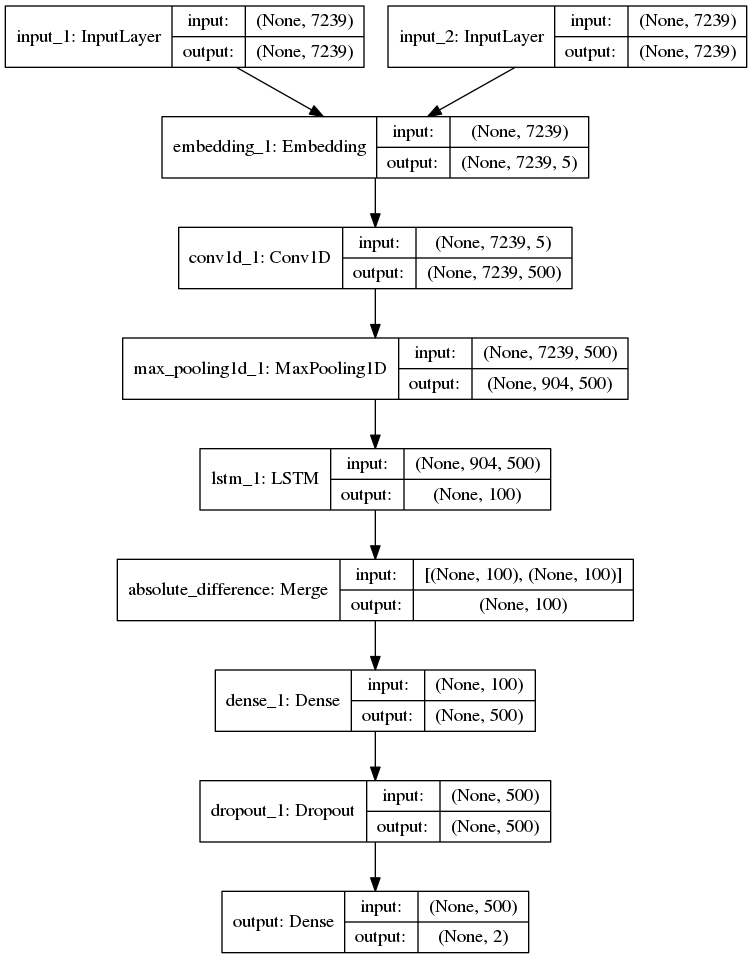
\includegraphics[width=\textwidth]{./pictures/experiments/network5.png}
    %\caption{Illustrate the structure of our fifth Siamese Neural Network.
        %Weights are shared by the embedding layers, the convolutional layer and
        %the LSTM layer. This Figure will be replaced by the new format when we
        %decide what that format is.}
    %\label{fig:network5}
%\end{figure}

%The network reached an accuracy of 0.89393 in epoch 18. The training and
%validation accuracies are shown in Figure \ref{fig:network_5_accuracies}. At the
%end of the training the network suddenly goes from about 90\% accuracy and back
%to 50\% accuracy. A reason for that happening could be that the optimizer
%overshot a target and therefore ended up with a worse result.

%\begin{figure}
    %\centering
    %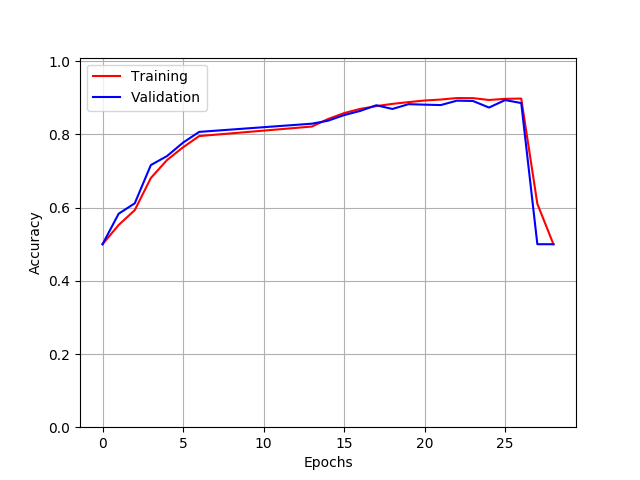
\includegraphics[width=0.5\textwidth]{./pictures/experiments/network_5_accuracies.png}
    %\caption{Shows the training and validation accuracies over the epochs of
        %training on the fifth iteration of our networks.}
    %\label{fig:network_5_accuracies}
%\end{figure}

%The students normally write their personal information in the beginning of
%assignments. Earlier we described that MaCom removed most of the names from
%the assignment. But they still contain information such as classes, dates and
%a different number of new line characters per student. We were suspicious
%that the networks still made use of some meta data from the texts so we tried
%training the network again but where we removed the 200 first characters from
%each text. Since most of the metadata are located in the beginning of the
%text we hoped that that would remove the problem. On this new dataset the
%best validation accuracy was obtained in epoch 3 with an accuracy of 0.53233.
%Clearly the network relied exclusively on the metadata in the beginning of
%the texts. We have shown the training and validation accuracies in Figure
%\ref{fig:network_5_accuracies_2}.

%\begin{figure}
    %\centering
    %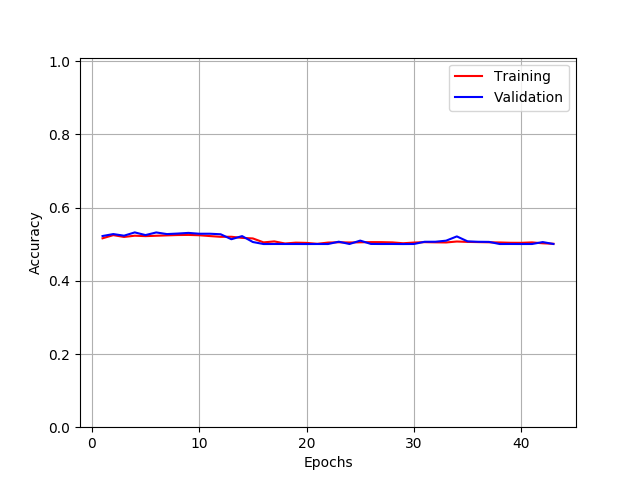
\includegraphics[width=0.5\textwidth]{./pictures/experiments/network_5_accuracies_2.png}
    %\caption{Shows the training and validation accuracies over the epochs of
        %training on the fifth iteration of our networks where we removed the 200
        %first characters.}
    %\label{fig:network_5_accuracies_2}
%\end{figure}


%\subsubsection{Siamese Neural Network - Iteration 6}
%\label{subsubsec:siamese_neuraon_network_iteration_6}

%In this iteration we trained our third network again but this time with the 200
%first characters removed like in Iteration 5. We wanted to see how much worse
%the network would perform now that we had hopefully removed some more personal
%information from what the network had available to look at. We have shown the
%training and validation accuracies in Figure \ref{fig:network_6_accuracies}. The
%best validation accuracy was obtained in epoch 57 with an accuracy of 0.74370.
%That means that we lost about 5\% accuracy by removing the first 200 characters.

%\begin{figure}
    %\centering
    %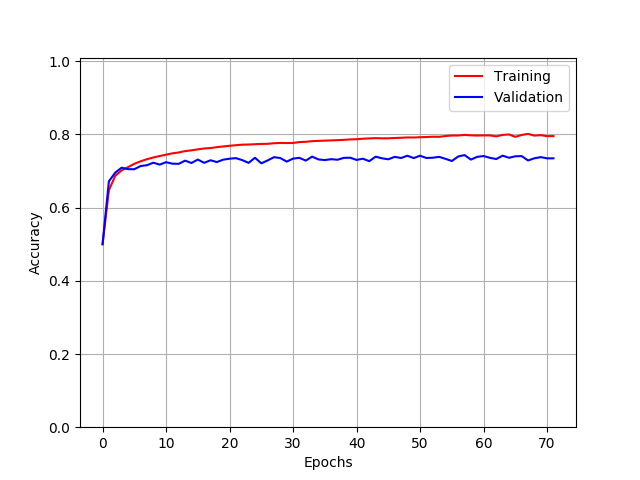
\includegraphics[width=0.5\textwidth]{./pictures/experiments/network_6_accuracies.png}
    %\caption{Shows the training and validation accuracies over the epochs of
        %training on the sixth iteration of our networks.}
    %\label{fig:network_6_accuracies}
%\end{figure}


%\subsubsection{Siamese Neural Network - Iteration 7}

%Since the overall performance and runtime of our network described in iterations
%5 did not perform very well, we chose a other route in terms of the \gls{RNN}'s.
%Using the approaches described in \cite{qian:2018} with some minor changes. A
%keras generated model can be seen in Figure \ref{fig:r_network6}.

%\begin{figure}
    %\centering
    %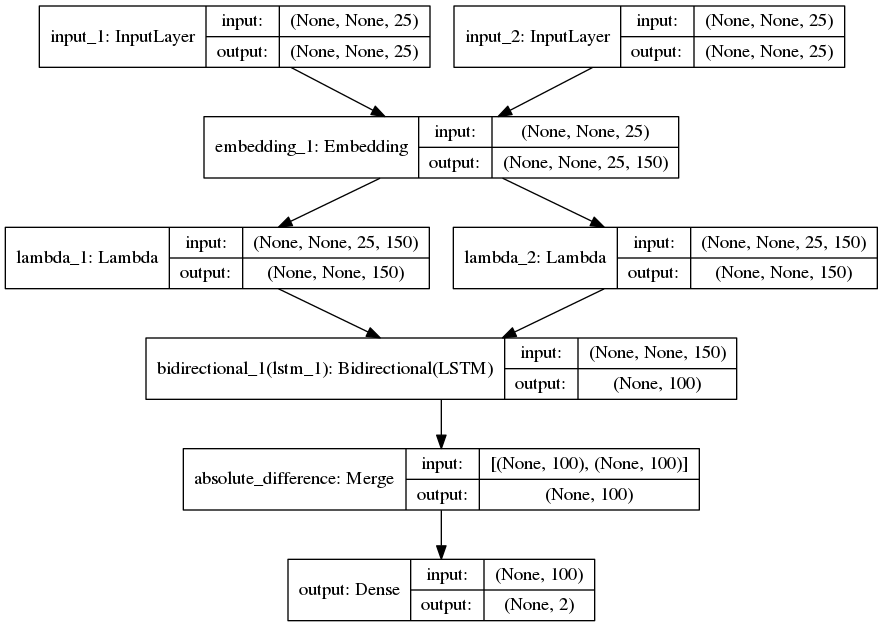
\includegraphics[width=0.5\textwidth]{./pictures/experiments/network6.png}
    %\caption{A keras generated model, showing the design of the \cite{qian:2018}
        %inspired network.}
    %\label{fig:r_network6}
%\end{figure}

%Contrary to previous networks we've produced, this network works on a higher
%linguistic level, by using words and sentences rather than characters. It does
%so by initially representing each text as a sequence of sequences. The outer
%sequence is a sentence and the inner sequence is the words of that sentence.
%We then proceed with representing each sentence as the sum of the embedded
%words in it. Each words is embedded to a vector of size 150, resulting in the
%summarized vector being the same size. Each of these summations are given to a
%bidirectional \gls{LSTM} layer, of 50 neurons. All this is done in a Siamese
%fashion so we have two branches of computation for each of the two texts given
%to the network, which are merged using the absolute difference. After this is
%done we simply feed this into a softmax dense layer to get the predictions.

%All sentences are padded and truncated to have length 25 and all texts in each
%batch are padded with 0 vectors to have the same length in sentences as the
%longest text in the batch. We use a bidirectional \gls{LSTM} to allow the
%network to use context from both sides of the current timestep.

%We have shown the training accuracy and validation accuracy in Figure
%\ref{fig:network_7_accuracies} (clearly we need to train some more epochs which
%should be running at the moment). The highest validation accuracy was obtained
%in epoch two with accuracy 0.92075.

%\begin{figure}
    %\centering
    %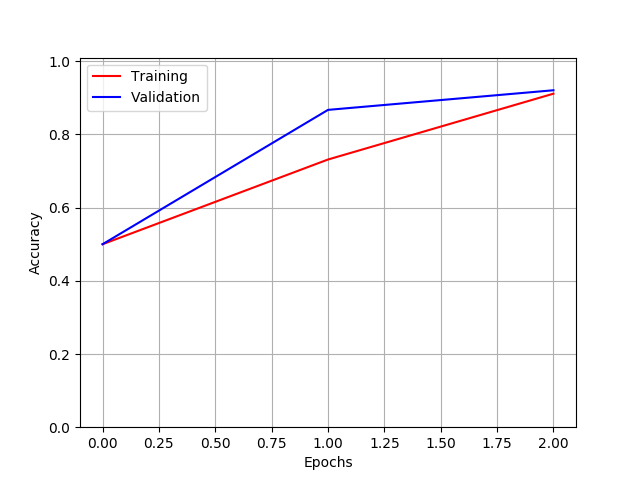
\includegraphics[width=0.5\textwidth]{./pictures/experiments/network_7_accuracies.png}
    %\caption{Shows the training and validation accuracies over the epochs of
        %training on the seventh iteration of our networks.}
    %\label{fig:network_7_accuracies}
%\end{figure}


%\subsubsection{Siamese Neural Network - Iteration 8}

%In this iteration we tried an extended version of the previous network. We used
%two bidirectional \gls{LSTM} layers on top of the word embeddings from before.
%Both of them returned sequences and we computed the final "features" by taking
%the average of the returned sequences giving us 50 numbers which indicated the
%author. We had huge problems with overfitting of the network on the training
%data authors. We have shown a graph of the training and validation accuracies
%in Figure \ref{fig:network_8_accuracies}.


%\subsubsection{Siamese Neural Network - Iteration 9}

%In this iteration we went back to using convolutional neural networks. Now we
%tried using both embedded words and embedded characters. We had a two
%convolutional layers for the characters, one looking at 8 characters and one
%looking at 4. For the words we had a convolutional layer looking at 8 words at a
%time. After the convolutional layer we had a max over time pooling layer for
%each of the filters and we combined the output for 2 texts with the absolute
%difference. We then had a densely connected network on top of that which learned
%from the features extracted. The dense network had 2 layers with 500 neurons in
%each. After that we had 30\% dropout and a softmax layer as usual.


\subsubsection{\glsdesc{rec-sent-NN}}
\label{subsubsec:rec_sent_nn}

After having attempted some convolutional approaches, as was just described,
we proceeded with some recurrent experiments as well. After having looked at
previous experiments made described in \cite{qian:2018}, which showed real
promise in terms of authorship attribution, we considered this a natural
extension of our convolutional approaches. Every \gls{RNN} experiment
was performed on the same data as the convolutional networks, and the
\textit{Embedding}, \textit{Feature Extraction}, \textit{Combining} and
\textit{Comparing} structure was used as for each of them too, and the best
model used can be seen depicted in figure \ref{fig:rec-sent-NN}. After
[TODO:EPOCH COUNT] epochs this network peaked with a validation accuracy of
[TODO:ACC]. When applied to the external validation set (C), it got a accuracy
of [TODO:ACC].

\begin{figure}
    \centering
    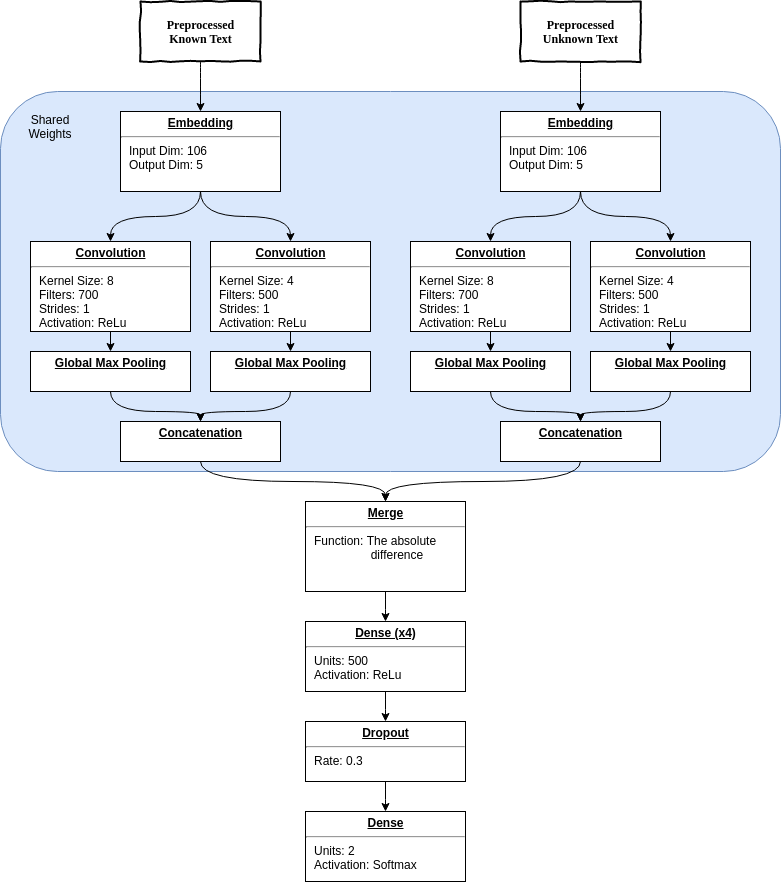
\includegraphics[width=\textwidth]{./pictures/experiments/conv_char_nn/model.png}
    \caption{The structure of network \gls{conv-char-NN}. Weights are
        shared by the embedding layers and the convolutional layers as shown by
        the blue box. The input to the network is at the top and the output is
        at the bottom. Information flows downwards through the layers. The final
        softmax layer produces a probability distribution over the two
        possibilities that the texts are either written by the same author or
        not.}
    \label{fig:conv-char-NN}
\end{figure}

\begin{figure}
\centering
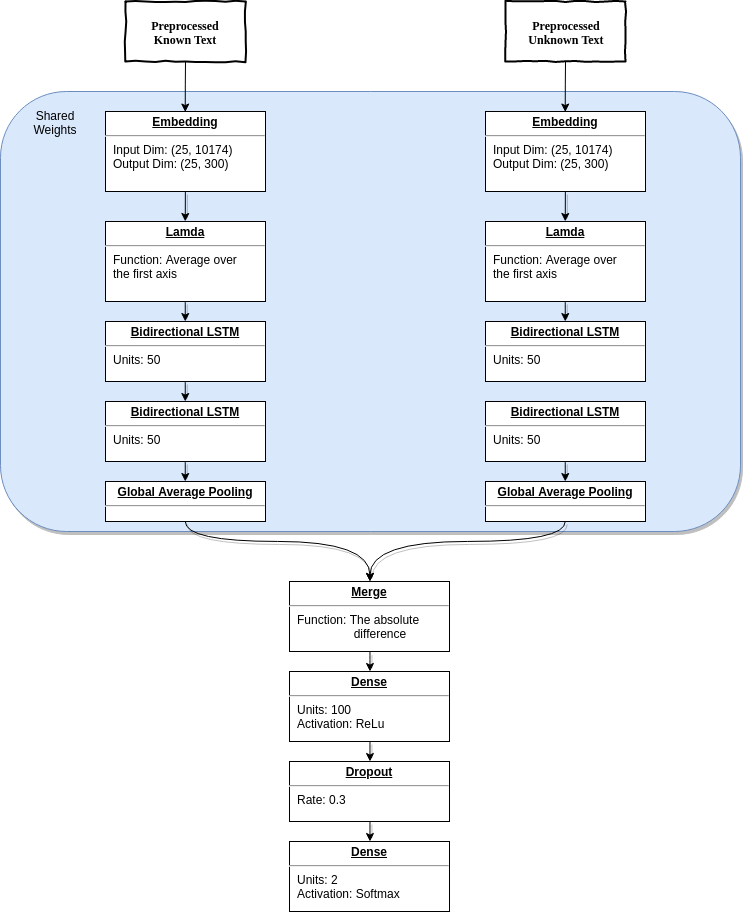
\includegraphics[width=\textwidth]{./pictures/experiments/rec_sent_nn/RNN_model.png}
\caption{The structure of network \gls{rec-sent-NN}. The weights are shared from
from the embedding layer all the way down to right before the two paths merge.
The lambda layer takes each sentence and averages along the first axis
causing the dimensionality to chance from (25, 300) to (, 300). The LSTM
layers are bidirectional meaning its runs through the layer from both directions,
resulting in an output dimensionality twice the unit count, 100 in this case.
\label{fig:rec-sent-NN}
\end{figure}

\begin{description}

    \item[Embedding:]

        In this recurrent network we started deviating in terms of our approach
        in the embedding layer. Like with the previous networks, this network
        is siamese as well. It is each training sample consists of two texts.
        As the title of this section suggests, this network works on the
        sentence level rather than the character level. It initially takes in
        a sequence of sequences. The outer sequence representing a sentence,
        and the sequence contained within the word associated with that.
        In order for the dimensionality to work, the amount of word in a
        sequence is padded or truncated so they consist of 25 words each.
        An amount which was chosen based on the analytics of the training
        data set. Contrary to the earlier networks created throughout our
        experiments, the embedded representations of these words were not
        trained as as part of the network. Pre-trained embedding produced by
        Facebook\footnote{\url{https://github.com/facebookresearch/fastText/blob
        /master/ pretrained-vectors.md}}, using the method described in
        \cite{bojanowski2016enriching} was used instead, resulting in each
        word being mapped to a 300 dimensional vector. At this point we have
        a sequence of sentences each containing a sequence of 300 dimensional
        word-embeddings. The network then proceeds to take the average of the
        word sequence contained within each sentence, resulting in each sentence
        being represented as the average of its' words.

    \item[Feature Extraction:]

        The feature extraction made in this network, of course bases itself
        on the usage recurrent layers, in this case the \gls{LSTM} layer
        which was described Section \ref{layer:LSTM}. Two of these are placed
        right after one another. Both of them consists of 50 units, and has
        the flag \textit{return\_sequence} set to true. This results in
        all time-steps of the \gls{RNN} being returned, rather than just
        the last one, giving us a sequence of outputs. We then proceed to
        combine all the returned sequences, using a global average pooling
        layer. Rather then using a simple ReLu, which was the activation
        function we used on most layers for the reason explained in Section
        \ref{subsubsec:activation_functions}, the LSTM layer makes use 2
        other activation functions. It makes use of the tahn activation
        function \eqref{eq:tanh} after the last time step, and the hard sigmoid
        activation function \eqref{eq:h_sig} after each individual time-step.
        This configuration is the default of the LSTM layer provided by keras,
        making the only change to the default parameters the number of units in
        the layer.

    \item[Combining:]

        Like the networks described in the earlier sections, the combinations
        of our two siamese paths, are done by taking the absolute difference of
        their two pooling outputs.

    \item[Decision:]

        The decision part of this network was kept quite simple. It simply
        consists of a single dense layer, of 100 units, which is then followed
        by a 0.3 dropout layer. The result of the dropout layer is then provided
        to the last dense layer, consisting of 2 neurons, and the soft-max
        activation function, thus mapping it into a usable probability space.
        Since two neurons were used to depict the final output, the loss
        function used for the network was categorical cross-entropy, paired with
        a \gls{Adam} optimizer with the learning rate of 0.0005, 50\% of the
        default value.

\end{description}

The path to this final design was a long one. The initial network designs
for our recurrent networks bases itself on a combination of the work done in
\ref{qian:2018} and our own character based convolutional network described in
Section \ref{subsubsec:conv_char_nn}. We simply replaced the feature extraction
component in the network, from convolutional layers to a single recurrent layer.
In addition that, the first \gls{RNN} network also used the cosine similarity
as its' method of combination on decision. It was when running this network,
that the main hindrance when using a character level recurrent network became
apparent, computation time. This first iteration of the network needed and
estimated 140 hours to run through a single epochs. Thus from this point on, the
goal became creating a recurrent network which would peak in accuracy run within
a feasible time-fame.

An attempt at this was the inclusion of a convolutional in the feature
extraction part of the network. This would be placed be the recurrent layers,
in an attempt to minimize the amount of data that was given to the current
layers. This did increase the runtime, but revealed the lack of learning the
network did, only getting a validation accuracy of [TODO:Insert ACC Here], at
its' peak. This was slightly increased when changing out the cosine similarity
approach with a series of dense layers instead, and using a bidirectional
\gls{LSTM} layer rather than a single \gls{GRU} layer. In other words the
problem lied in the lack of performance to be assumed to lie in inclusion of the
convolutional layer, which precedes the recurrent one. It was however due to
this convolutional layer that running any of the recurrent networks was possible
within an acceptable time-frame, so another approach had to be used.

This secondary approach to limiting the run-time used, came in the form of
changing the linguistic level out network worked at. Against inspired by
\ref{qian:2018}, we elevated our network from using the characters of the texts,
to using the sentences. This sentence representation was achieved by doing as
was described in the \textbf{Embedding} part above. This approach yielded only
significantly decreased the runtime to around $1.5$ hours. But it also revealed
the reason why a recurrent network might not be the best choice for a task like
this. The validation error throughout training the network was not very high
compared to earlier convolutional network, and after running it through the
prediction system it became obvious that the network was really good a learning
individual author. In a task such as this, were generalization is a key factor,
a network that does this individual learning really suffers when it comes to
accuracy. This lead to the final network described above. This network included
an extra bidirectional \gls{LSTM} layer for added complexity, and the 0.3
dropout for extra generalization.

% TODO Results


\subsubsection{\glsdesc{conv-char-word-NN}}
\label{subsubsec:conv_char_word_nn}


\subsection{Prediction System}

Our prediction system has several hyperparameters we have to choose to get
the best results. We recall that MaCom wanted a system that had an accusation
error of less than 10\%. We can use the threshold parameter $\theta$ in the
prediction system to control how many people we accuse. The best parameters
for the prediction system is those parameters that gives the highest accuracy
subject to the constraint that the accusation error should be less than 10\%.
To tune the parameters we use a validation dataset $V$ consisting of a set of
tuples $(\alpha, t_u)$ where $\alpha$ is a candidate author and $t_u$ is a text
of unknown authorship. None of the authors in $V$ has been seen by the networks
during training and none of the texts $t_u$ has been seen by the networks during
training. The parameters that maximize the accuracy subject to the bounded
accusation error is the same as the parameters that minimize the error rate
subject to the bounded accusation error. That optimization problem is,

\begin{equation}
    \label{eq:prediction_system_minimization}
    \begin{aligned}
        & \underset{\theta, w}{\text{minimize}}
        & & \sum_{(\alpha, t_u) \in V} \left|
            P(f, w, T_\alpha \setminus \{t_u\}, t_u, \theta) -
            \mathbbm{1}_{T_\alpha}(t_u)
        \right| \\
        & \text{subject to}
        & & \frac{\sum_{(\alpha, t_u) \in V} \mathbbm{1}_{T_\alpha}(t_u) \cdot
            \left(1 - P(f, w, T_\alpha \setminus \{t_u\}, t_u, \theta)\right)}
{\sum_{(\alpha, t_u) \in V} (1 - P(f, w, T_\alpha \setminus \{t_u\}, t_u, \theta)} <
            \frac{1}{10}
    \end{aligned}
\end{equation}

In the optimization problem we fix the network $f$ we validate. The expression
we minimize is the number of errors made in prediction over the validation set
$V$. Consider a problem $(\alpha, t_u) \in V$ where $t_u \in T_\alpha$. Then we
know that $\mathbbm{1}_{T_\alpha}(t_u) = 1$ from the definition of the indicator
function then if the prediction system returns the correct result 1 we have,

\begin{equation}
    e = \left|
        P(f, w, T_\alpha \setminus \{t_u\}, t_u, \theta) -
        \mathbbm{1}_{T_\alpha}(t_u)
    \right| = |1 - 1| = 0,
\end{equation}

and if the prediction system returns the incorrect result 0 we have,

\begin{equation}
    e = \left|
        P(f, w, T_\alpha \setminus \{t_u\}, t_u, \theta) -
        \mathbbm{1}_{T_\alpha}(t_u)
    \right| = |0 - 1| = 1.
\end{equation}

Similarly for a problem $(\alpha, t_u) \in V$ where $t_u \notin T_\alpha$ we
know that $\mathbbm{1}_{T_\alpha}(t_u) = 0$ from the definition of the indicator
function. Then if the prediction system returns the correct result 0 we have,

\begin{equation}
    e = \left|
        P(f, w, T_\alpha \setminus \{t_u\}, t_u, \theta) -
        \mathbbm{1}_{T_\alpha}(t_u)
    \right| = |0 - 0| = 0, \end{equation}

and if the prediction system returns the incorrect result 1 we have,

\begin{equation}
    e = \left|
        P(f, w, T_\alpha \setminus \{t_u\}, t_u, \theta) -
        \mathbbm{1}_{T_\alpha}(t_u)
    \right| = |1 - 0| = 1.
\end{equation}

That is the expression we minimize is 0 whenever there is no error and 1
whenever there is an error. So we minimize the number of errors we make. The
subject to expression makes sure that the fraction of false accusations we make
is less than $10\%$ of the accusations we make. The expression should be read
as,

\begin{equation}
    \frac{\textit{false accusations}}{\textit{total accusations}} < \frac{1}{10}
\end{equation}

Consider the numerator of the fraction on the left hand side,

\begin{equation}
    \textit{false accusations} = \sum_{(\alpha, t_u) \in V}
    \mathbbm{1}_{T_\alpha}(t_u) \cdot
    \left(1 - P(f, w, T_\alpha \setminus \{t_u\}, t_u, \theta)\right).
\end{equation}

For a $(\alpha, t_u) \in V$ where $t_u \in T_\alpha$ we have that
$\mathbbm{1}_{T_\alpha}(t_u) = 1$ then if $P$ is correct it returns 1 and we
get,

\begin{equation}
    \mathbbm{1}_{T_\alpha}(t_u) \cdot
    \left(1 - P(f, w, T_\alpha \setminus \{t_u\}, t_u, \theta)\right) =
    1 \cdot (1 - 1) = 0,
\end{equation}

and if $P$ is incorrect and returns 0 we have,

\begin{equation}
    \mathbbm{1}_{T_\alpha}(t_u) \cdot
    \left(1 - P(f, w, T_\alpha \setminus \{t_u\}, t_u, \theta)\right) =
    1 \cdot (1 - 0) = 1.
\end{equation}

Similarly for a $(\alpha, t_u) \in V$ where $t_u \in T_\alpha$ we have that
$\mathbbm{1}_{T_\alpha}(t_u) = 0$ and therefore the expression is always
0. Therefore the expression is 1 whenever we have a false accusation and 0
otherwise. The right hand side of the inequality simply counts the number of
accusations by inverting the output of $P$ and divides that by 10. So the
condition makes sure that only 10\% of the accusations we make are false
accusations.

We have run our prediction system on several of the networks we trained as
part of our experiments. For each of the networks we present several graphs
showing their performance for different weights and thresholds and we report
the best configuration for that network. The dataset we use to tune $\theta$
and the weight function $w$ are F. The set consists of 2000 previously unseen
authors. From them we generate two problems for each author meaning that we
end up with 4000 different problems. For each of the authors we generate a
positive sample by taking the newest text as the unknown text and a negative
sample by choosing a random text from some other author in the set. That is
we have a 0.5 split between positive and negative samples. We also tried our
prediction system on another validation set. In the real world it has been
estimated that 4\% of turn ins for the \gls{SRP} are written by "ghost writers"
\footnote{https://politiken.dk/indland/uddannelse/art5603163/Gymnasieelever-\%C2
\% BBSnyderi-beviser-hvor-vanvittig-betydningsfuld-SRP-er-blevet\%C2\%AB}. We
therefore also wanted to find the $\theta$ and $w$ for a validation set with
only 4\% negative samples instead of 50\% negative samples. We generated 2000
positive samples as before and then for each sample we added a negative sample
with a 4\% chance.


\subsubsection{\glsdesc{conv-char-NN}}

The first network we tuned hyperparameters for were the network presented
in Figure \ref{fig:conv-char-NN}. The network used only convolutions on the
character level to extract features and used a dense network to decide whether
or not the texts were written by the same author. We have shown the accuracy
and accusation error for the dataset containing 50\% negatives in Figure
\ref{fig:conv-char-NN-pred-50} and for the dataset containing 4\% negatives in
Figure \ref{fig:conv-char-NN-pred-4}.

\begin{figure}
    \centering
    \textbf{Prediction System Results for 0.5 Split}\par\medskip
    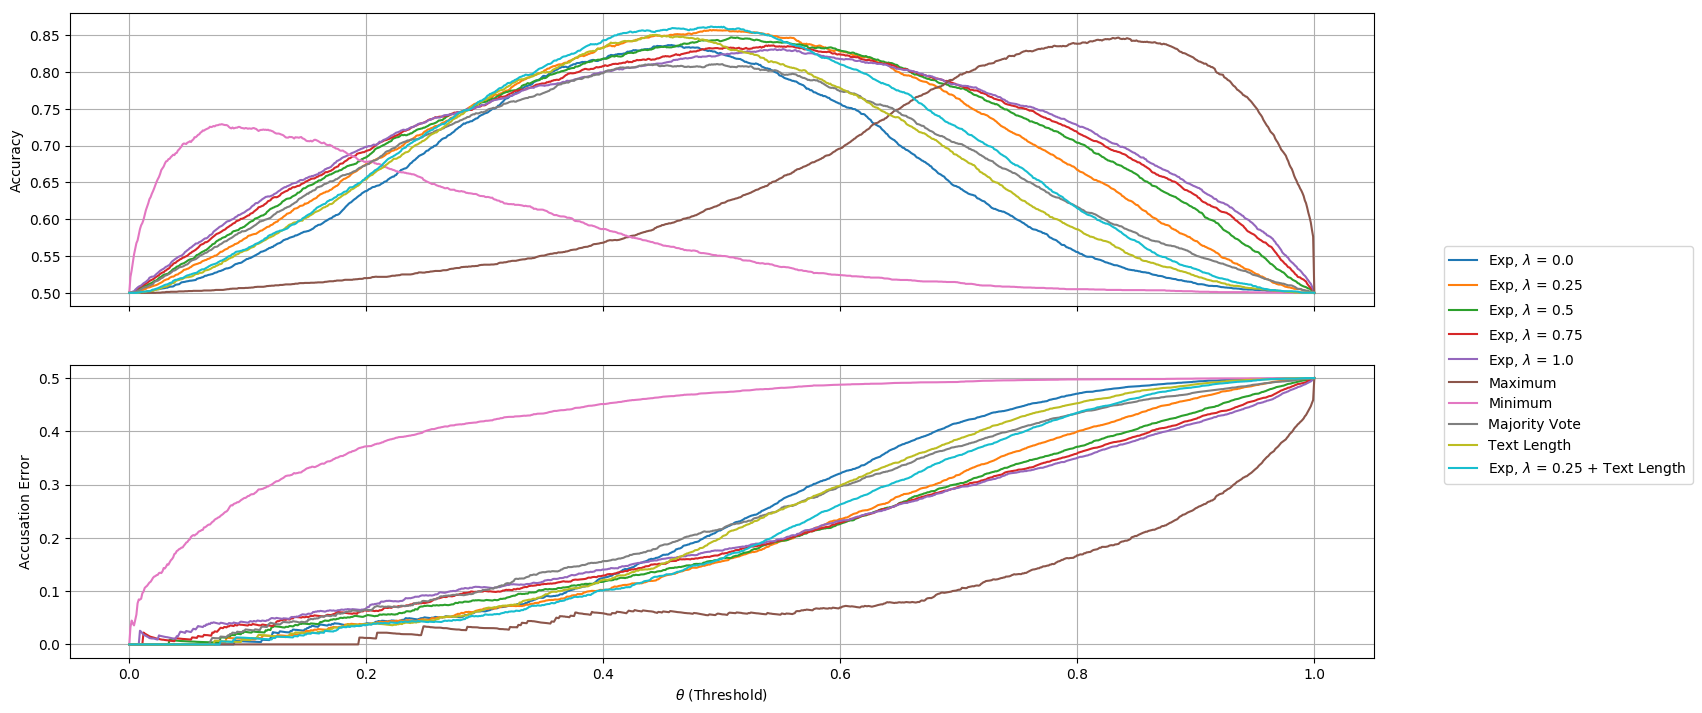
\includegraphics[width=\textwidth]{./pictures/experiments/conv_char_nn/prediction_system_50.png}
    \caption{Results of running the prediction system with the network described
        in Section \ref{subsubsec:conv_char_nn} on a validation dataset with
        50\% positive samples and 50\% negative samples. In the upper graph we
        show the accuracies obtained as a function of $\theta$ for different
        weights $w$. At the bottom we have shown the accusation error as a
        function $\theta$ again with one line for each weight. We can see that
        as the threshold increases and we accuse more people of cheating the
        accusation error rises.}
    \label{fig:conv-char-NN-pred-50}
\end{figure}

\begin{figure}
    \centering
    \textbf{Prediction System Results for 0.04 Split}\par\medskip
    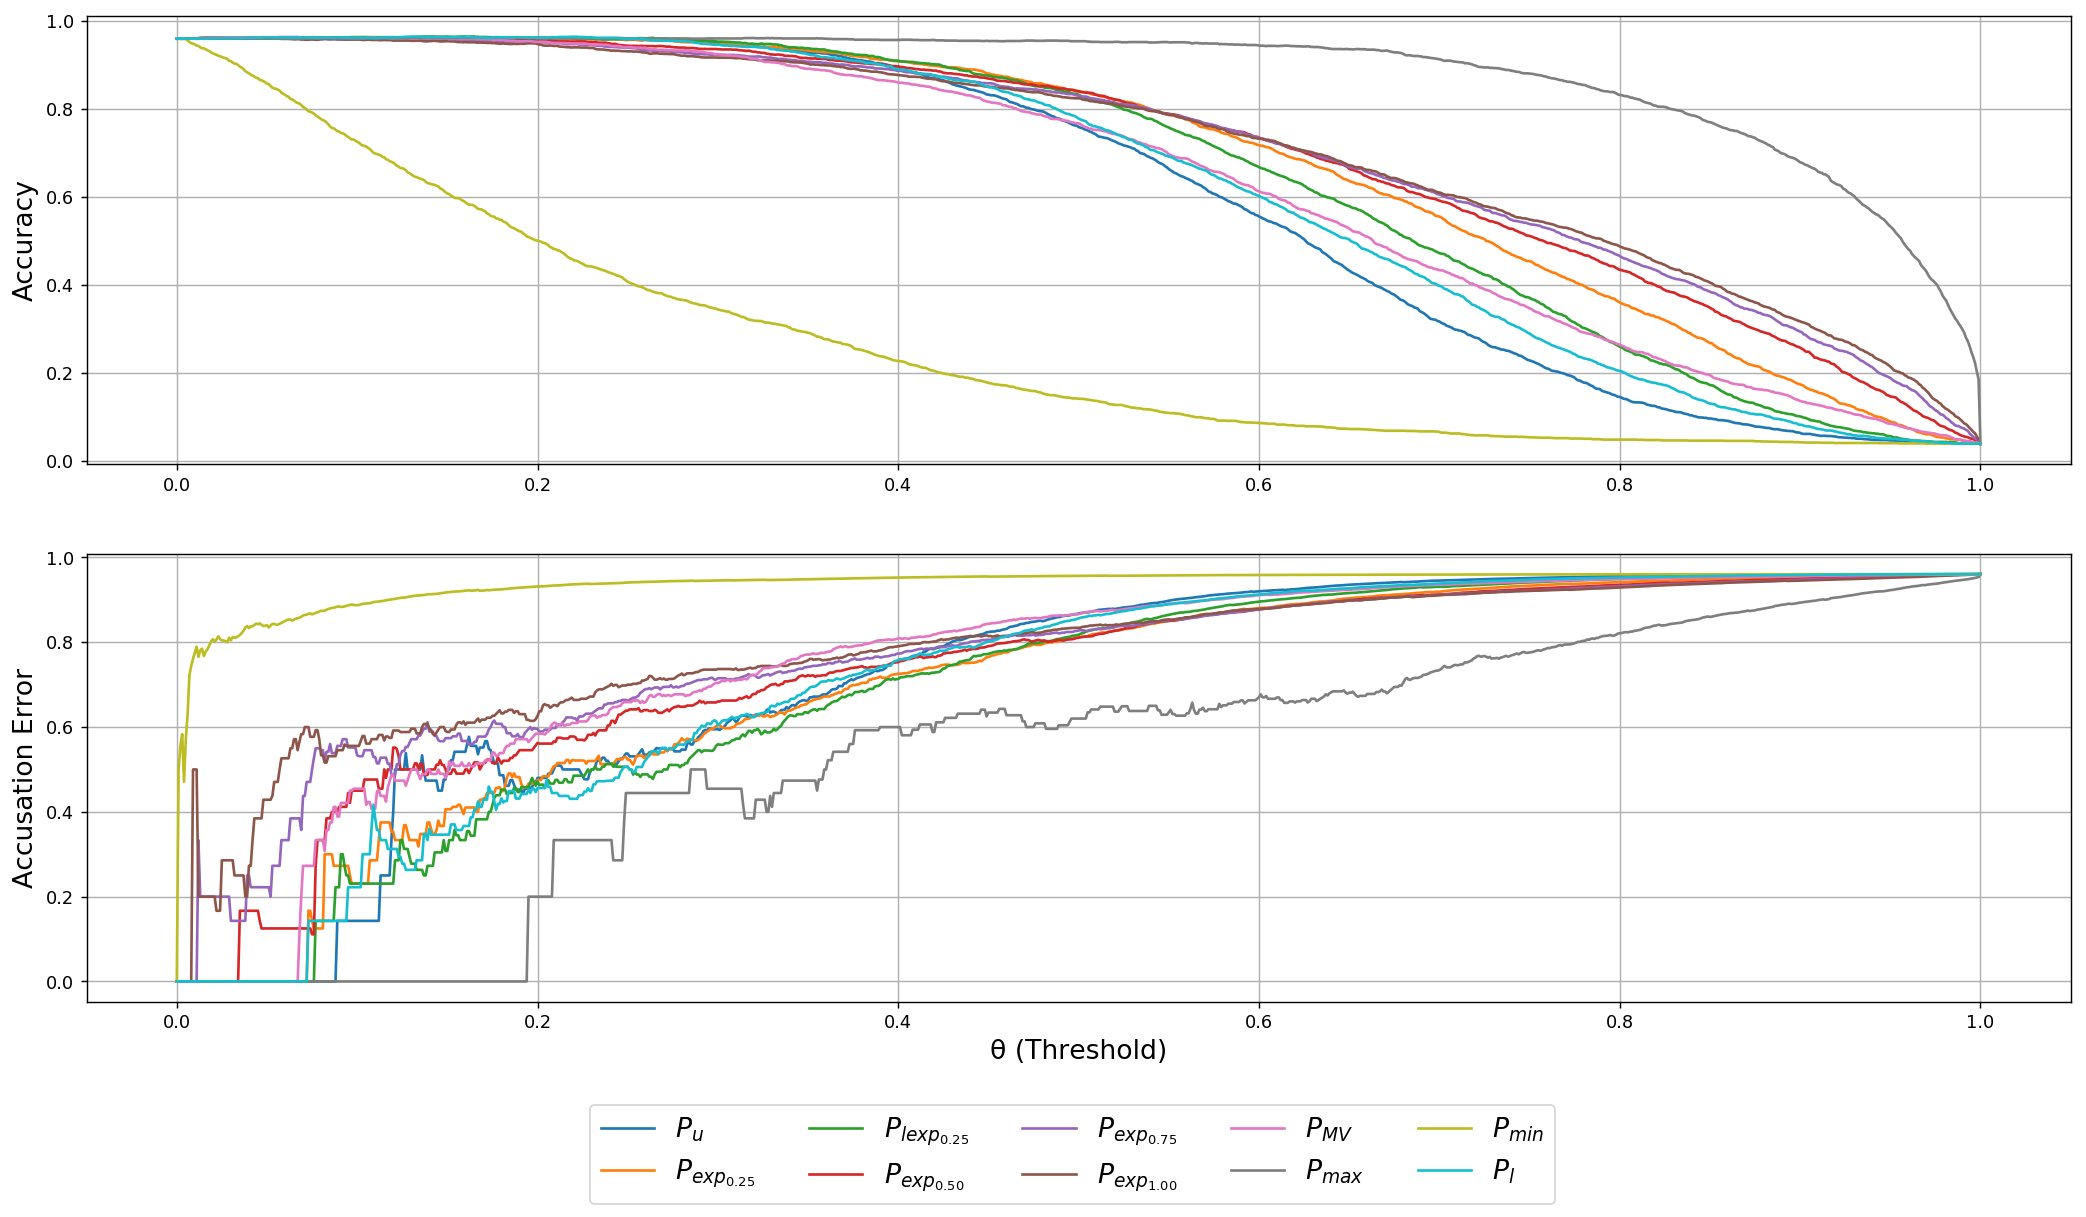
\includegraphics[width=\textwidth]{./pictures/experiments/conv_char_nn/prediction_system_04.png}
    \caption{Results of running the prediction system with the network described
        in Section \ref{subsubsec:conv_char_nn} on a validation dataset with
        96\% positive samples and 4\% negative samples. In the upper graph we
        show the accuracies obtained as a function of $\theta$ for different
        weights $w$. At the bottom we have shown the accusation error as a
        function $\theta$ again with one line for each weight. We can see that
        as the threshold increases and we accuse more people of cheating the
        accusation error rises.}
    \label{fig:conv-char-NN-pred-4}
\end{figure}

The best configuration for the 0.5 split were using the Exponential Norm Weight
function with $\lambda = 0.25$ and using the threshold $\theta = 0.395398$.
That configuration obtained an accusation error of 9.9761\% and an accuracy of
83.5168 \%. The configuration had 1507 \gls{TN}s, 1832 \gls{TP}s, 167 \gls{FN}s
and 492 \gls{FP}s. The best configuration for the 0.04 split were using the
Exponential Norm Weight function with $\lambda = 0.5$ and using the threshold
$\theta = 0.076101$. That configuration obtained an accusation error of 5.5556
\% and an accuracy of 96.8750 \%. The configuration had 17 \gls{TN}s, 1998
\gls{TP}s, 1 \gls{FN}s and 64 \gls{FP}s.


\subsubsection{\glsdesc{conv-char-word-NN}}

The second network we tuned hyperparameters for were the network presented
in Figure TODO. The network used convolutions on the character level and
word level to extract features and used a dense network to decide whether or
not the texts were written by the same author. We have shown the accuracy
and accusation error for the dataset containing 50\% negatives in Figure
\ref{fig:conv-char-word-NN-pred-50} and for the dataset containing 4\%
negatives in Figure \ref{fig:conv-char-word-NN-pred-4}.

\begin{figure}
    \centering
    \textbf{Prediction System Results for 0.5 Split}\par\medskip
    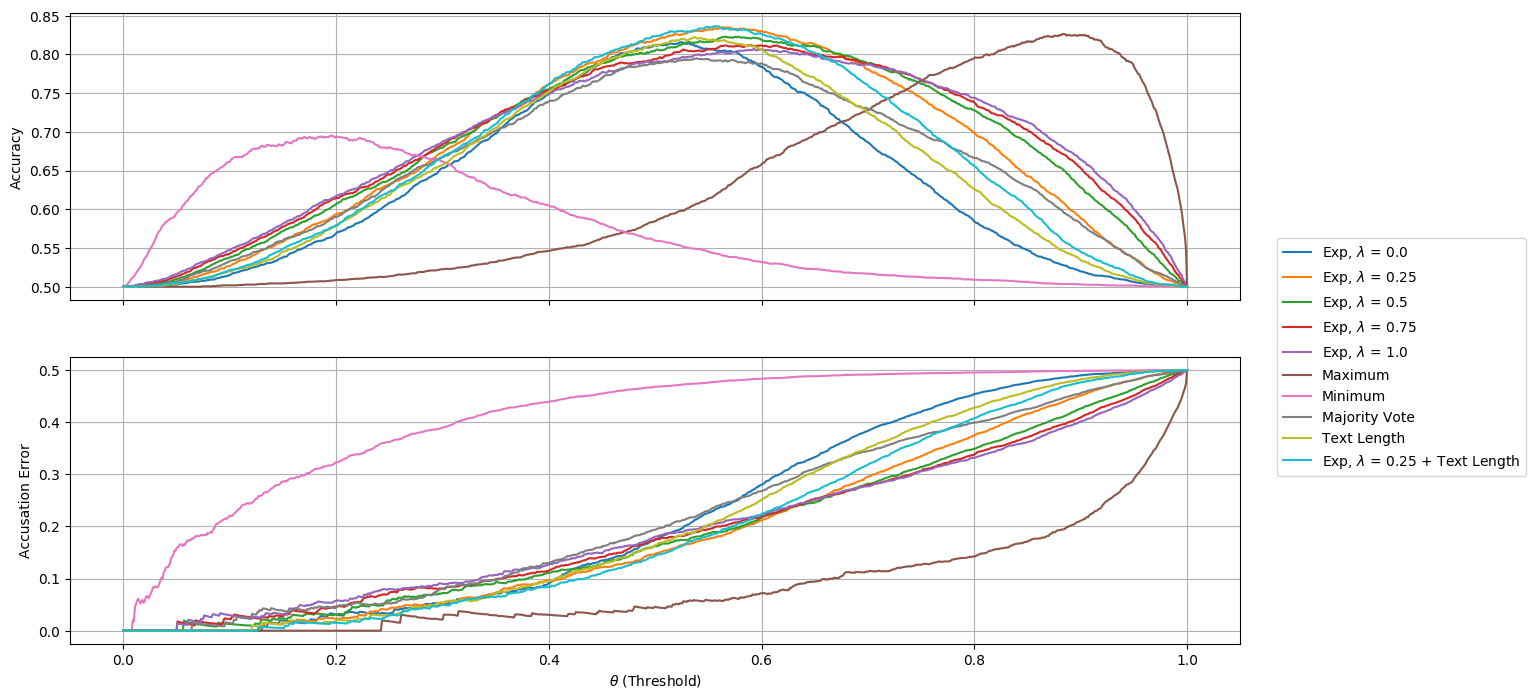
\includegraphics[width=\textwidth]{./pictures/experiments/conv_char_word_nn/prediction_system_50.png}
    \caption{Results of running the prediction system with the network described
        in Section \ref{subsubsec:conv_char_word_nn} on a validation dataset
        with 50\% positive samples and 50\% negative samples. In the upper graph
        we show the accuracies obtained as a function of $\theta$ for different
        weights $w$. At the bottom we have shown the accusation error as a
        function $\theta$ again with one line for each weight. We can see that
        as the threshold increases and we accuse more people of cheating the
        accusation error rises.}
    \label{fig:conv-char-word-NN-pred-50}
\end{figure}

\begin{figure}
    \centering
    \textbf{Prediction System Results for 0.04 Split}\par\medskip
    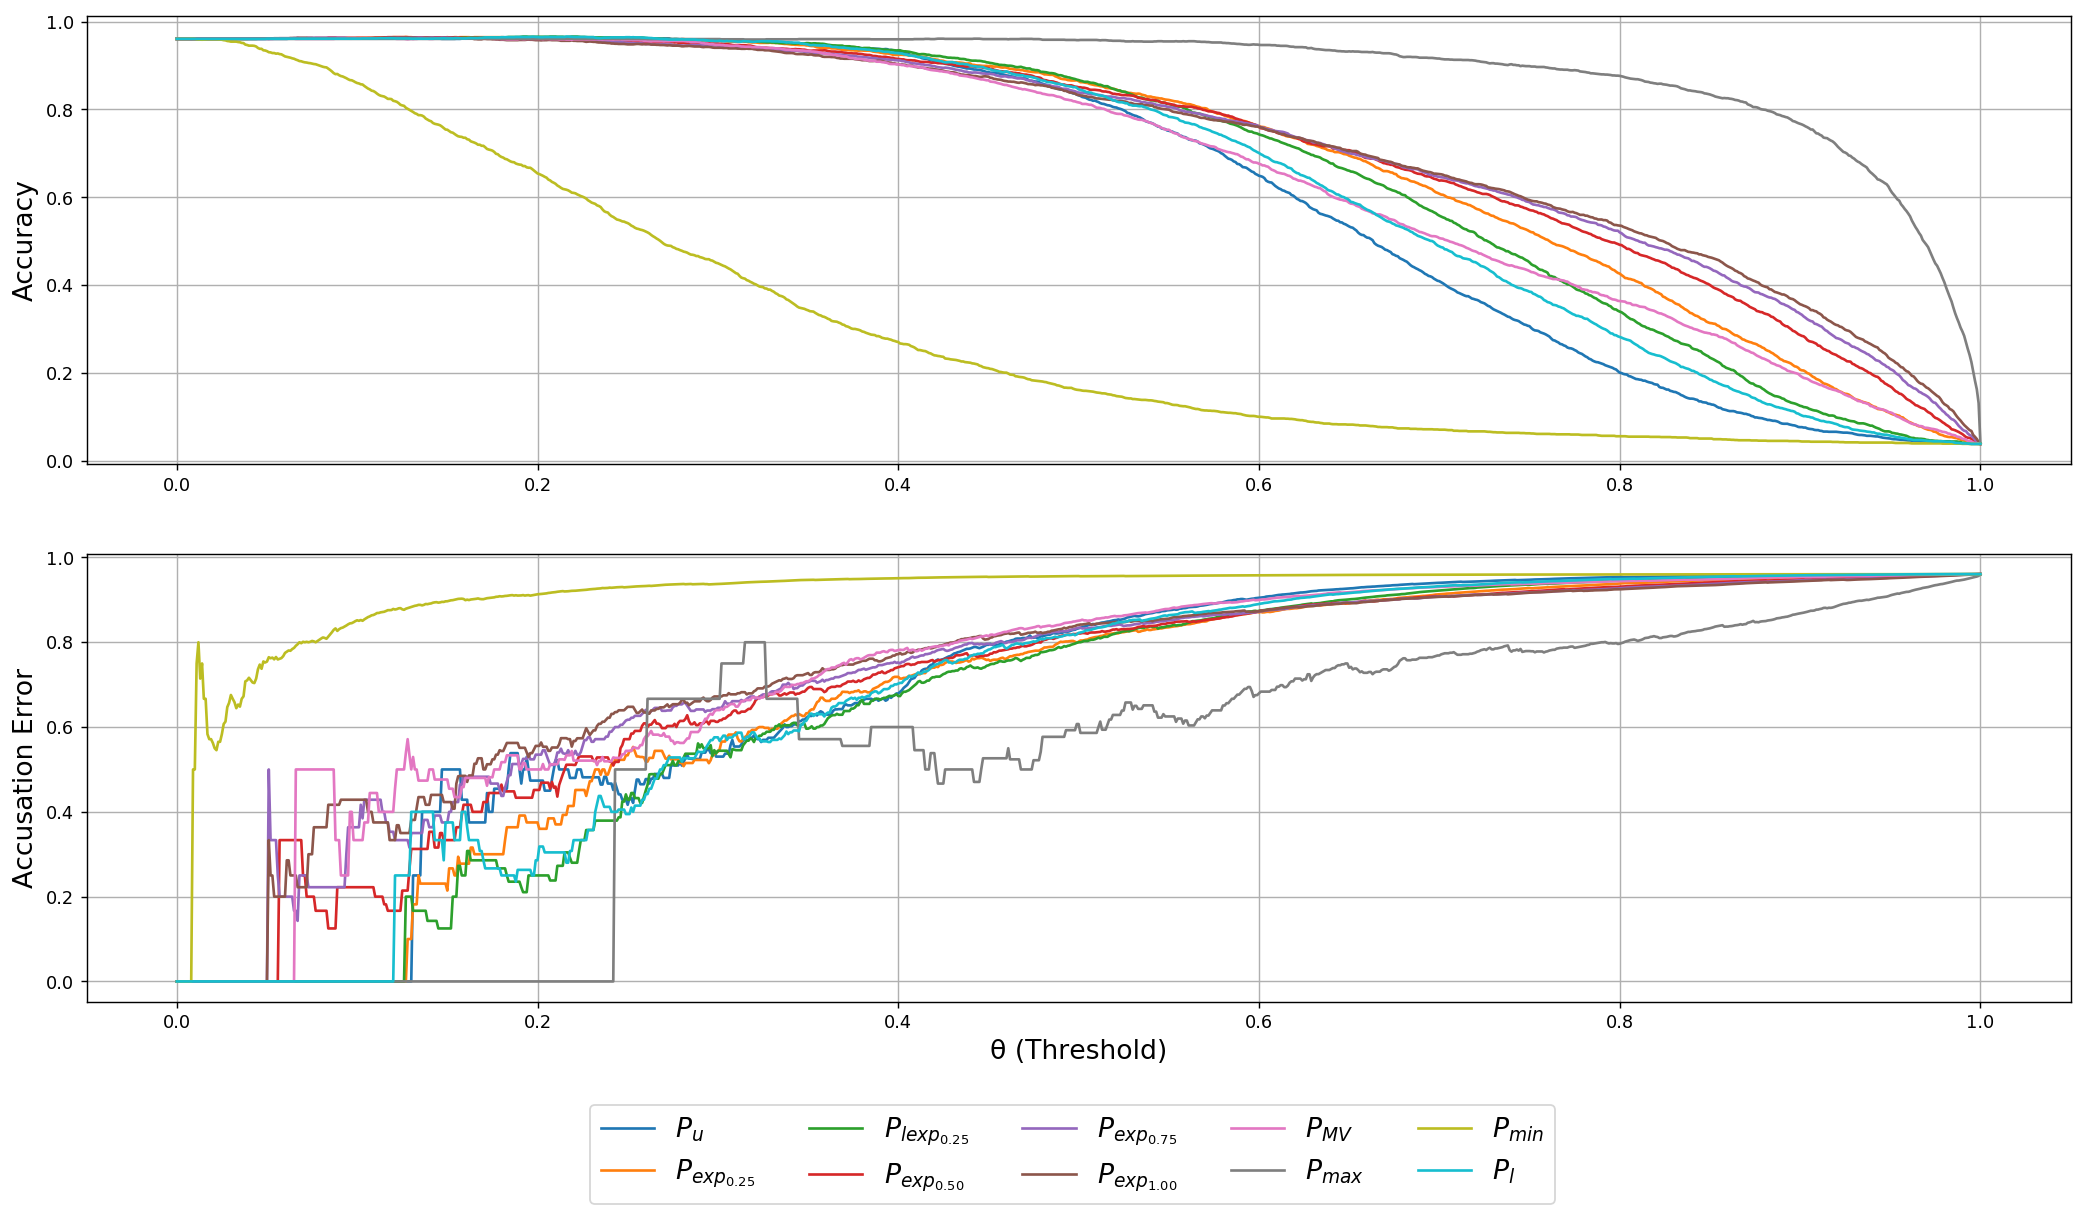
\includegraphics[width=\textwidth]{./pictures/experiments/conv_char_word_nn/prediction_system_04.png}
    \caption{Results of running the prediction system with the network described
        in Section \ref{subsubsec:conv_char_word_nn} on a validation dataset
        with 96\% positive samples and 4\% negative samples. In the upper graph
        we show the accuracies obtained as a function of $\theta$ for different
        weights $w$. At the bottom we have shown the accusation error as a
        function $\theta$ again with one line for each weight. We can see that
        as the threshold increases and we accuse more people of cheating the
        accusation error rises.}
    \label{fig:conv-char-word-NN-pred-4}
\end{figure}

The best configuration for the 0.5 split were using the Exponential Norm Weight
function with $\lambda = 0.25$ and using the threshold $\theta = 0.376832$.
That configuration obtained an accusation error of 9.9766\% and an accuracy of
75.6878 \%. The configuration had 1155 \gls{TN}s, 1871 \gls{TP}s, 128 \gls{FN}s
and 844 \gls{FP}s. The best configuration for the 0.04 split were using the
Maximum Weight function and using the threshold $\theta = 0.235470$. That
configuration obtained an accusation error of 0 \% and an accuracy of 96.9022
\%. The configuration had 3 \gls{TN}s, 1999 \gls{TP}s, 0 \gls{FN}s and 64
\gls{FP}s.
